% Created by tikzDevice version 0.7.0 on 2014-07-31 11:04:19
% !TEX encoding = UTF-8 Unicode
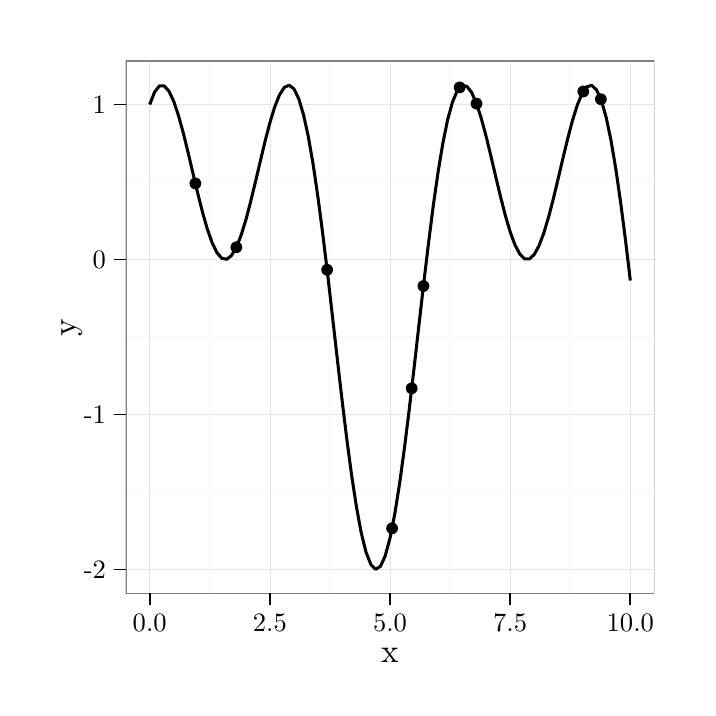
\begin{tikzpicture}[x=1pt,y=1pt]
\definecolor[named]{fillColor}{rgb}{1.00,1.00,1.00}
\path[use as bounding box,fill=fillColor,fill opacity=0.00] (0,0) rectangle (238.49,238.49);
\begin{scope}
\path[clip] (  0.00,  0.00) rectangle (238.49,238.49);
\definecolor[named]{drawColor}{rgb}{1.00,1.00,1.00}
\definecolor[named]{fillColor}{rgb}{1.00,1.00,1.00}

\path[draw=drawColor,line width= 0.6pt,line join=round,line cap=round,fill=fillColor] (  0.00,  0.00) rectangle (238.49,238.49);
\end{scope}
\begin{scope}
\path[clip] ( 35.42, 34.03) rectangle (226.45,226.45);
\definecolor[named]{fillColor}{rgb}{1.00,1.00,1.00}

\path[fill=fillColor] ( 35.42, 34.03) rectangle (226.45,226.45);
\definecolor[named]{drawColor}{rgb}{0.98,0.98,0.98}

\path[draw=drawColor,line width= 0.6pt,line join=round] ( 35.42, 70.75) --
	(226.45, 70.75);

\path[draw=drawColor,line width= 0.6pt,line join=round] ( 35.42,126.74) --
	(226.45,126.74);

\path[draw=drawColor,line width= 0.6pt,line join=round] ( 35.42,182.72) --
	(226.45,182.72);

\path[draw=drawColor,line width= 0.6pt,line join=round] ( 65.81, 34.03) --
	( 65.81,226.45);

\path[draw=drawColor,line width= 0.6pt,line join=round] (109.23, 34.03) --
	(109.23,226.45);

\path[draw=drawColor,line width= 0.6pt,line join=round] (152.64, 34.03) --
	(152.64,226.45);

\path[draw=drawColor,line width= 0.6pt,line join=round] (196.06, 34.03) --
	(196.06,226.45);
\definecolor[named]{drawColor}{rgb}{0.90,0.90,0.90}

\path[draw=drawColor,line width= 0.2pt,line join=round] ( 35.42, 42.76) --
	(226.45, 42.76);

\path[draw=drawColor,line width= 0.2pt,line join=round] ( 35.42, 98.74) --
	(226.45, 98.74);

\path[draw=drawColor,line width= 0.2pt,line join=round] ( 35.42,154.73) --
	(226.45,154.73);

\path[draw=drawColor,line width= 0.2pt,line join=round] ( 35.42,210.71) --
	(226.45,210.71);

\path[draw=drawColor,line width= 0.2pt,line join=round] ( 44.10, 34.03) --
	( 44.10,226.45);

\path[draw=drawColor,line width= 0.2pt,line join=round] ( 87.52, 34.03) --
	( 87.52,226.45);

\path[draw=drawColor,line width= 0.2pt,line join=round] (130.93, 34.03) --
	(130.93,226.45);

\path[draw=drawColor,line width= 0.2pt,line join=round] (174.35, 34.03) --
	(174.35,226.45);

\path[draw=drawColor,line width= 0.2pt,line join=round] (217.76, 34.03) --
	(217.76,226.45);
\definecolor[named]{drawColor}{rgb}{0.00,0.00,0.00}

\path[draw=drawColor,line width= 1.1pt,line join=round] ( 44.10,210.71) --
	( 45.84,215.19) --
	( 47.58,217.42) --
	( 49.31,217.48) --
	( 51.05,215.54) --
	( 52.79,211.82) --
	( 54.52,206.63) --
	( 56.26,200.31) --
	( 58.00,193.26) --
	( 59.73,185.86) --
	( 61.47,178.54) --
	( 63.21,171.68) --
	( 64.94,165.63) --
	( 66.68,160.70) --
	( 68.42,157.15) --
	( 70.15,155.15) --
	( 71.89,154.80) --
	( 73.63,156.12) --
	( 75.36,159.05) --
	( 77.10,163.43) --
	( 78.84,169.04) --
	( 80.57,175.61) --
	( 82.31,182.79) --
	( 84.05,190.20) --
	( 85.78,197.44) --
	( 87.52,204.12) --
	( 89.26,209.82) --
	( 90.99,214.19) --
	( 92.73,216.90) --
	( 94.47,217.70) --
	( 96.20,216.39) --
	( 97.94,212.85) --
	( 99.67,207.07) --
	(101.41,199.10) --
	(103.15,189.10) --
	(104.88,177.30) --
	(106.62,164.01) --
	(108.36,149.62) --
	(110.09,134.54) --
	(111.83,119.25) --
	(113.57,104.21) --
	(115.30, 89.93) --
	(117.04, 76.86) --
	(118.78, 65.44) --
	(120.51, 56.04) --
	(122.25, 48.99) --
	(123.99, 44.52) --
	(125.72, 42.78) --
	(127.46, 43.83) --
	(129.20, 47.64) --
	(130.93, 54.07) --
	(132.67, 62.91) --
	(134.41, 73.86) --
	(136.14, 86.56) --
	(137.88,100.59) --
	(139.62,115.48) --
	(141.35,130.75) --
	(143.09,145.93) --
	(144.83,160.53) --
	(146.56,174.13) --
	(148.30,186.33) --
	(150.04,196.80) --
	(151.77,205.29) --
	(153.51,211.62) --
	(155.25,215.72) --
	(156.98,217.58) --
	(158.72,217.29) --
	(160.46,215.03) --
	(162.19,211.04) --
	(163.93,205.63) --
	(165.67,199.17) --
	(167.40,192.03) --
	(169.14,184.62) --
	(170.88,177.34) --
	(172.61,170.59) --
	(174.35,164.71) --
	(176.08,160.00) --
	(177.82,156.70) --
	(179.56,154.97) --
	(181.29,154.91) --
	(183.03,156.50) --
	(184.77,159.69) --
	(186.50,164.29) --
	(188.24,170.09) --
	(189.98,176.78) --
	(191.71,184.03) --
	(193.45,191.44) --
	(195.19,198.62) --
	(196.92,205.15) --
	(198.66,210.66) --
	(200.40,214.77) --
	(202.13,217.18) --
	(203.87,217.63) --
	(205.61,215.95) --
	(207.34,212.03) --
	(209.08,205.88) --
	(210.82,197.55) --
	(212.55,187.23) --
	(214.29,175.16) --
	(216.03,161.66) --
	(217.76,147.12);
\definecolor[named]{fillColor}{rgb}{0.00,0.00,0.00}

\path[fill=fillColor] (207.13,212.64) circle (  2.13);

\path[fill=fillColor] (138.77,108.17) circle (  2.13);

\path[fill=fillColor] (162.19,211.04) circle (  2.13);

\path[fill=fillColor] (200.77,215.44) circle (  2.13);

\path[fill=fillColor] (143.00,145.13) circle (  2.13);

\path[fill=fillColor] (156.10,216.91) circle (  2.13);

\path[fill=fillColor] (131.68, 57.58) circle (  2.13);

\path[fill=fillColor] ( 75.41,159.14) circle (  2.13);

\path[fill=fillColor] ( 60.60,182.20) circle (  2.13);

\path[fill=fillColor] (108.20,151.00) circle (  2.13);
\definecolor[named]{drawColor}{rgb}{0.50,0.50,0.50}

\path[draw=drawColor,line width= 0.6pt,line join=round,line cap=round] ( 35.42, 34.03) rectangle (226.45,226.45);
\end{scope}
\begin{scope}
\path[clip] (  0.00,  0.00) rectangle (238.49,238.49);
\definecolor[named]{drawColor}{rgb}{0.00,0.00,0.00}

\node[text=drawColor,anchor=base east,inner sep=0pt, outer sep=0pt, scale=  0.96] at ( 28.31, 39.45) {-2};

\node[text=drawColor,anchor=base east,inner sep=0pt, outer sep=0pt, scale=  0.96] at ( 28.31, 95.44) {-1};

\node[text=drawColor,anchor=base east,inner sep=0pt, outer sep=0pt, scale=  0.96] at ( 28.31,151.42) {0};

\node[text=drawColor,anchor=base east,inner sep=0pt, outer sep=0pt, scale=  0.96] at ( 28.31,207.41) {1};
\end{scope}
\begin{scope}
\path[clip] (  0.00,  0.00) rectangle (238.49,238.49);
\definecolor[named]{drawColor}{rgb}{0.00,0.00,0.00}

\path[draw=drawColor,line width= 0.6pt,line join=round] ( 31.15, 42.76) --
	( 35.42, 42.76);

\path[draw=drawColor,line width= 0.6pt,line join=round] ( 31.15, 98.74) --
	( 35.42, 98.74);

\path[draw=drawColor,line width= 0.6pt,line join=round] ( 31.15,154.73) --
	( 35.42,154.73);

\path[draw=drawColor,line width= 0.6pt,line join=round] ( 31.15,210.71) --
	( 35.42,210.71);
\end{scope}
\begin{scope}
\path[clip] (  0.00,  0.00) rectangle (238.49,238.49);
\definecolor[named]{drawColor}{rgb}{0.00,0.00,0.00}

\path[draw=drawColor,line width= 0.6pt,line join=round] ( 44.10, 29.77) --
	( 44.10, 34.03);

\path[draw=drawColor,line width= 0.6pt,line join=round] ( 87.52, 29.77) --
	( 87.52, 34.03);

\path[draw=drawColor,line width= 0.6pt,line join=round] (130.93, 29.77) --
	(130.93, 34.03);

\path[draw=drawColor,line width= 0.6pt,line join=round] (174.35, 29.77) --
	(174.35, 34.03);

\path[draw=drawColor,line width= 0.6pt,line join=round] (217.76, 29.77) --
	(217.76, 34.03);
\end{scope}
\begin{scope}
\path[clip] (  0.00,  0.00) rectangle (238.49,238.49);
\definecolor[named]{drawColor}{rgb}{0.00,0.00,0.00}

\node[text=drawColor,anchor=base,inner sep=0pt, outer sep=0pt, scale=  0.96] at ( 44.10, 20.31) {0.0};

\node[text=drawColor,anchor=base,inner sep=0pt, outer sep=0pt, scale=  0.96] at ( 87.52, 20.31) {2.5};

\node[text=drawColor,anchor=base,inner sep=0pt, outer sep=0pt, scale=  0.96] at (130.93, 20.31) {5.0};

\node[text=drawColor,anchor=base,inner sep=0pt, outer sep=0pt, scale=  0.96] at (174.35, 20.31) {7.5};

\node[text=drawColor,anchor=base,inner sep=0pt, outer sep=0pt, scale=  0.96] at (217.76, 20.31) {10.0};
\end{scope}
\begin{scope}
\path[clip] (  0.00,  0.00) rectangle (238.49,238.49);
\definecolor[named]{drawColor}{rgb}{0.00,0.00,0.00}

\node[text=drawColor,anchor=base,inner sep=0pt, outer sep=0pt, scale=  1.20] at (130.93,  9.03) {x};
\end{scope}
\begin{scope}
\path[clip] (  0.00,  0.00) rectangle (238.49,238.49);
\definecolor[named]{drawColor}{rgb}{0.00,0.00,0.00}

\node[text=drawColor,rotate= 90.00,anchor=base,inner sep=0pt, outer sep=0pt, scale=  1.20] at ( 17.30,130.24) {y};
\end{scope}
\end{tikzpicture}
